\chapter{Desenvolvimento} \label{desenvolvimento}

% \section{Ferramentas Utilizadas}
% \begin{enumerate}
%     \item LTSpice XVII x64 - Analog Devices Inc.
% \end{enumerate}

Antes de iniciar o desenvolvimento, foi realizada uma extensa pesquisa sobre missões com \textit{CubeSats} para buscar referências e teve por objetivo entender os requisitos e especificações de outras missões bem sucedidas e usar essas informações como um guia para o EPS que será desenvolvido no LODESTAR. 

A tabela \ref{history_table} mostra as missões, ano de deploy e um resumo das soluções utilizadas.

\begin{table}
\centering
\caption{Missões anteriores com \textit{Cubesats}}
\label{history_table}
\begin{tabular}{|l|l|l|l|} 
\hline
\multicolumn{1}{|c|}{Nome} & \multicolumn{1}{c|}{Tipo} & \multicolumn{1}{c|}{Ano} & \multicolumn{1}{c|}{Implementação do EPS}  \\ 
\hline
Cute 1.7+                  & Demonstração              & 2008                     &  Implementação do MPPT, centralizado  \\ 
\hline
SNAP-1                     & Demonstração              & 2000                     &  Implementação do MPPT, parcialmente distribuído  \\
\hline
ESTCube-1                  & Científico                & 2013                     &  Controladores MPPT, centralizado     \\ 
\hline
SwissCube                  & Observação                & 2009                     &  Implementação do MPPT, centralizado  \\
\hline
\end{tabular}
\end{table}

O CUTE \cite{cute1_ref} (Cubical  Tóquio  Tech  Engineering  Satellite-I) é um projeto cooperativo do LSS (Laboratory for Space Systems) e o SRTL (Space Robotics and Teleoperations Laboratory), ambos de Tóquio. O computador de bordo foi implementado com um processador Hitachi NPD-20JWL e executava o sistema operacional Windows CE.NET. O  projeto  educacional  de  baixo  custo  usava componentes COTS para uma missão de demonstração tecnológica, o projeto teve diversões lançamentos (Cute-I, Cute 1.7+ APD, Cute 1.7+ APD II). 

O SNAP-1 \cite{snap1_ref} foi o primeiro nanossatélite desenvolvido no Reino Unido pela Surrey Space Centre (SSC) e Surrey Satellite Tecnology Ltd (SSTL) e serviu como veículo de teste para demonstração da nova tecnologia que estava surgindo, ele foi um dos pioneiros dessa nova filósofia de design e mostrou que era possível construir um nanossatélite rapidamente e com custo baixo, utilizando peças COTS.

SamSat-218D \cite{samsat218_ref} foi um nanossatélite desenvolvido na \textit{Samara State Aerospace University}, lançado em 2015, e foi criado com o objetivo de ser uma plataforma de testes para tecnologias de navegação e controle. Além disso, o projeto foi utilizado para testar um OBC experimental, que empregava os processadores ATXmega 128U4 e LPC4357 DualCore, testar o controle de voo em condições anormais e novos painéis solares.

ESTCube-1 \cite{estcube1_ref} foi um \textit{cubesat} 1U lançado pelo foguete Vega VV02. Desenvolvido por uma força tarefa de 4 universidades, tinha o objetivo científico de realizar um prova de conceito de medição e demonstração da tecnologia da tecnologia de velas solares elétricas. Para o OBC um STMicroelectronics STM32F103 (ARM 32bits) foi escolhido para fazer os cálculos.

Cat-2 \cite{cat2_ref} foi um projeto de \textit{cubesat} 6U desenvolvido na \textit{Universitat Politècnica de Catalunya} e iniciado em 2009 para lançar um nanossatélite plataforma para um instrumento GNSS-R (do inglês, \textit{Global Navigation Satellite Systems Reflectometry}) que realizaria altimetria oceânica. A computação de bordo ficou a cargo de um ARM7TDMI.  

O SwissCube-1, \cite{swisscube_ref} foi um \textit{cubesat} suíço científico de tamanho 1U, operado pela Ecole Polytechnique Fédérale de Lausanne (EPFL) para realizar pesquisas sobre o \textit{nightglow} (fenômeno de brilho   noturno na atmosfera terrestre) e também para desenvolver tecnologia para futuras naves espaciais. A  computação  de  bordo utilizava um processador ARM7TDMI e o sistema operacional de tempo real FreeRTOS.


%\section{Módulos do Cubesat}

\section{Análise de consumo energético da missão}

Um dos pontos centrais para um projeto de EPS é dimensionar o \textit{payload} e os outros subsistemas para o pior cenário de consumo. O EPS deve ser capaz de manter o \textit{cubesat} em funcionamento quando esse cenário estiver presente. A tabela \ref{tab:requisites_modules} mostra os consumos máximos absolutos separados por módulo.

\begin{table}[!ht]
    \centering
    \begin{tabular}{l|ccc}
        Subsistema & Corrente & Tensão & Potência \\
        \hline
        Atuador magnético & \SI{900}{\milli\ampere} & \SI{5}{\volt} & \SI{4,5}{\watt}\\
        On board computer (OBC) & \SI{160}{\milli\ampere} & \SI{5}{\volt} & \SI{0.8}{\watt}\\
        Transceiver UHF & \SI{1.2}{\ampere} & \SI{3.3}{\volt} & \SI{3.96}{\watt}\\
        AD\&CS & \SI{2}{\milli\ampere} & \SI{3.3}{\volt} & \SI{6.6}{\milli\watt}\\
        \hline
        Total \SI{3.3}{\volt} & ~\SI{1.4}{\ampere} & - & \SI{4}{\watt}\\
        Total \SI{5}{\volt} & ~\SI{1.06}{\ampere} & - & \SI{5.3}{\watt}\\ \hline
        Total & ~\SI{2.5}{\ampere} & - & \SI{9.3}{\watt}\\
    \end{tabular}
    \caption{Requisitos de potência para cada subsistema}
    \label{tab:requisites_modules}
\end{table}

A pesquisa pelos outros EPSs lançados nos mostrou algumas opções com relação a arquitetura. A primeira decisão é sobre quem é responsável por fazer a regulação e distribuição das linhas, ou seja, se o EPS deve centralizar a regulação das linhas e já fornecer a alimentação para os diversos módulos já com a tensão e carga requeridas por cada um deles. A outra opção é distribuir essa responsabilidade entre os módulos de forma que cada é responsável por regular as tensões necessárias para o funcionamento interno daquele módulo. Usualmente, quando o EPS é responsável pela regulação das linhas de tensão existe também alguma interface que permita aos módulos controlar qual linha está ligada em um dado momento, normalmente o protocolo $I^{2}C$ é o escolhido para essa comunicação.

A segunda decisão arquitetural envolve a implementação da técnica MPPT, em uma das arquiteturas as células solares são colocadas em regime MPPT com um conversor DC/DC, um microcontrolador é usado para ajustar o \textit{Duty Cycle} de uma \textit{PWM - Pulse Width Modulation} e colocar esse ponto baseado na tensão e corrente da célula solar. A saída do conversor DC/DC é conectada a um circuito de proteção da bateria, responsável por parar o carregamento caso esta esteja totalmente carregada. Esse módulo também é responsável pela proteções de \textit{under-voltage} e \textit{over-current}, o que consiste em basicamente desligar as cargas para proteger a saúde da bateria, dado que existe um limite até é possível que ela seja descarregada. A outra opção existente é utilizar um controlador MPPT completo, onde no mesmo circuito integrado estão reunidos,

Após isso, a saída protegida é regulada para multiplas linhas que podem alimentar um ou mais subsistemas. 

Baseado nessa arquitetura e nas especificações do padrão Cubesat, a figura \ref{fig:block_diagram} mostra o diagrama de blocos da implementação proposta:

% TODO: Aumentar o tamanho dessa imagem.
% DONE: Imagem rotacionada e ocupando uma página completa 
\noindent
\begin{minipage}{\linewidth}
\makebox[\linewidth]{
    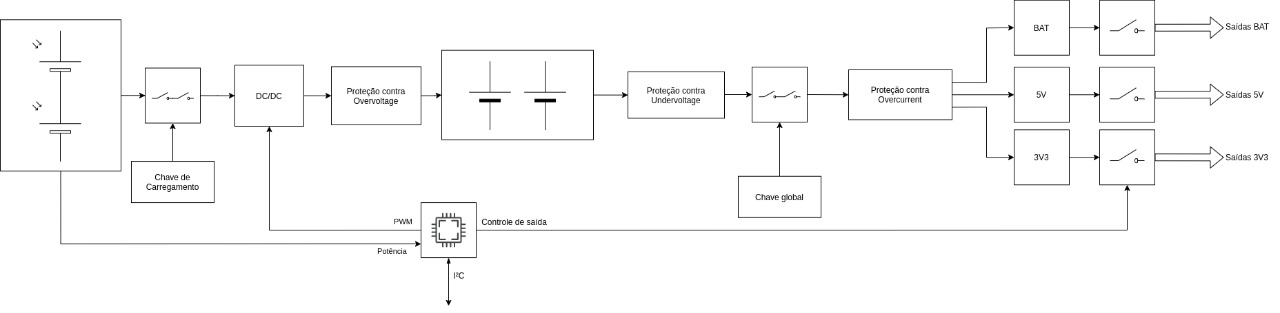
\includegraphics[angle=270,keepaspectratio=true, scale=0.55]{imagens/DiagramaBlocos.jpeg}}
\captionof{figure}{Diagrama de blocos proposto para o EPS}
\label{fig:block_diagram}
\end{minipage}

\subsection{Tarefas e \textit{Power Budget}}

Após levantar os consumos de cada módulo, o próximo passo é construir um \textit{power budget} baseado nas tarefas que o \textit{cubesat} precisa realizar ao longo de um ciclo.  

Alguns blocos da figura \ref{fig:block_diagram}, tais como as células solares e baterias foram escolhidas baseadas no \textit{power budget} disponível. Segue abaixo o \textit{power budget} estimado para a missão, detalhando cada um dos componentes e seus consumos, baseado nisso, e usando as informações da órbita, é possível determinar o número minímo de baterias e de células solares para conseguir carregar com sucesso o conjunto de baterias durante um ciclo. A figura \ref{fig:power_budget} mostra o \textit{power budget}:

\noindent
\begin{minipage}{\linewidth}
\makebox[\linewidth]{
    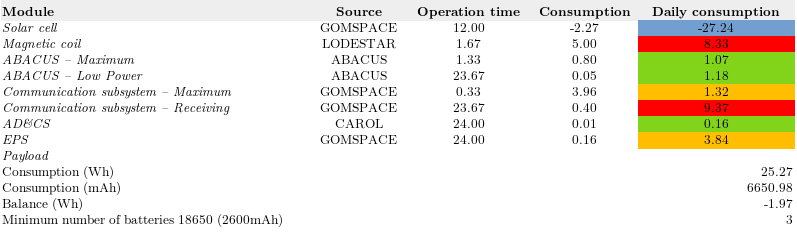
\includegraphics[keepaspectratio=true, scale=0.5]{imagens/powerbudget.png}}
\captionof{figure}{\textit{Power budget} estimado para o EPS}
\label{fig:power_budget}
\end{minipage}

% TODO: Corrigir arrendondamento na planilha

As seguintes premissas foram consideradas na construção dessa tabela:

\begin{enumerate}
    \item O sistema de comunicação irá operar por um período máximo de 20 minutos e permanecerá em modo de recepção durante o restante do ciclo.
    \item O consumo do atuador magnético está modelado para funcionar com pulsos de 1 minuto em potência máxima, é assumido que haverão 100 pulsos durante o ciclo.
    \item O computador de bordo (OBC) estará em modo ativo por no máximo 1 hora e durante o tempo que estiver ocorrendo transmissões, no total de 1 hora e 20 minutos.
\end{enumerate}

Com esse \textit{power budget}, a menor célular solar (1U) da GOMSPACE é usada como referência. Essa célula solar é capaz de prover até \SI{27}{\watt}. Note que usada apenas essa célula, o \textit{budget} ainda fica com um saldo negativo, o que significa que estamos consumindo menos energia do que a que conseguimos adquirir, porém essa margem ainda é pequena. Portanto, mais células solares devem ser usadas para prover uma quantidade segura de energia.

Conhecer os consumos dos módulos permitiu calcular quantas baterias, aqui estamos utilzando os modelos 18650 como referência, para manter o nanossatelite alimentado durante um ciclo. Os modelos de baterias 18650 são largamente utilizados nos EPS pela padronização de tamanho e segurança. No modelo referência da GOMSPACE temos \SI{2600}{\milli\ampere\hour}, ou seja, para conseguir suprir o consumo de \SI{6650}{\milli\ampere\hour}, pelo menos três dessas baterias.

\section{Circuito de carga da bateria}

Uma das tarefas cruciais para o projeto do circuito de carga da bateria é escolher o conversor DC/DC que fará a interface entre o painel solar e a bateria, o que nos permite aplicar a técnica de MPPT. Para cumprir essa tarefa, foi realizada uma busca pelos conversores disponíveis comercialmente e abaixo apresentaremos os resultados e as métricas utilizadas para escolha.


    
\subsection{Cenário de simulação}


% \noindent
% \begin{minipage}{\linewidth}
% \makebox[\linewidth]{
%     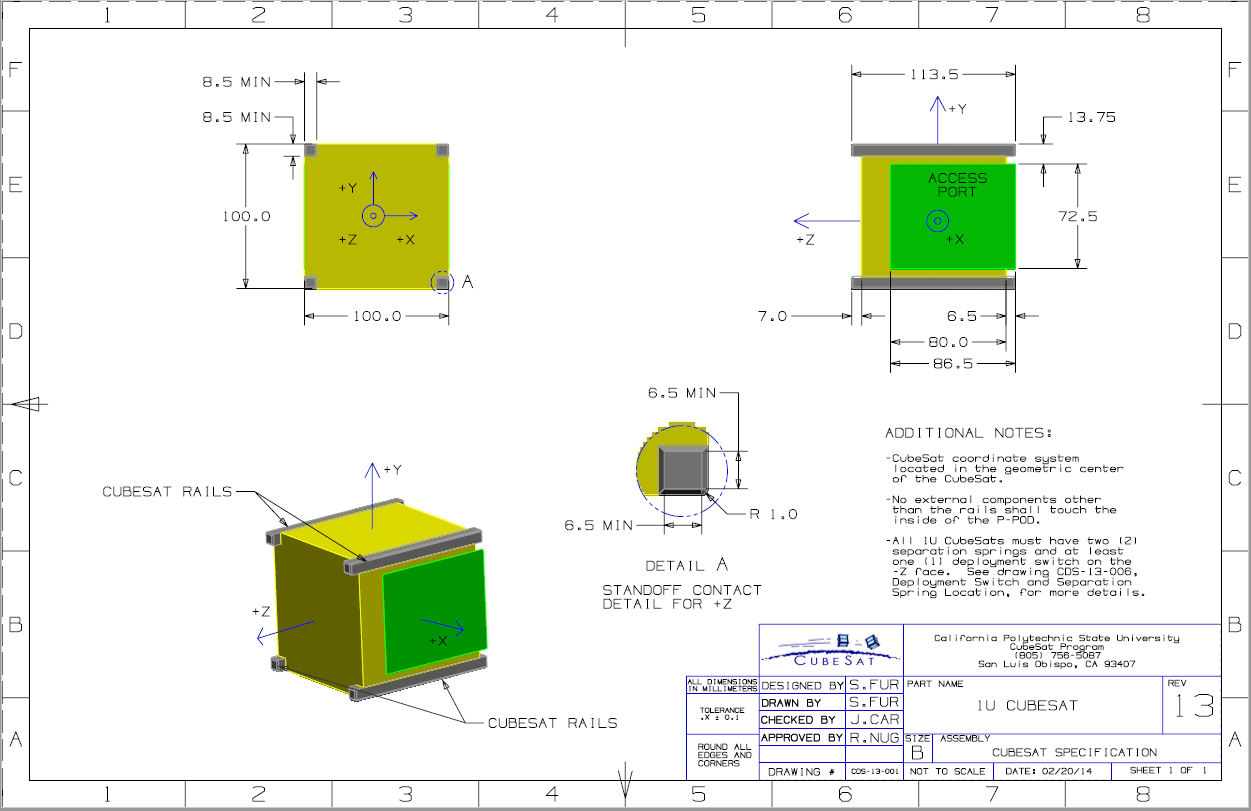
\includegraphics[keepaspectratio=true, scale=0.5]{imagens/Cubesat-diagram.png}}
% \captionof{figure}{Especificações de dimensionamento para um Cubesat 1U}
% \label{cubesat1U_dimensions}
% \end{minipage}

% A Tabela \ref{tabela1} a seguir apresenta os tipos de \textit{chunk} de um pacote do protocolo.

% \begin{table}[ht!]
%   \begin{center}
%   \setlength{\belowcaptionskip}{10pt} % espao entre caption e tabela
%   \footnotesize {
%       \begin{tabular}{|p{4cm}|p{9cm}|}
% 	  \hline
% 	  \textbf{Nome} & \textbf{Função} \\
% 	  \hline
% 	  Iniciar & Usado para iniciar uma associação \\
% 	  \hline
% 	  Confirmacao & Segunda mensagem de uma configuração de uma associação\\
% 	  \hline
% 	  Mensagem & Terceira mensagem de uma configuração de uma associação\\
% 	  \hline
% 	  Cookie & Quarta mensagem de uma configuração de uma associação\\
% 	  \hline
% 	  Dados & Dados da aplicação\\
% 	  \hline
%       \end{tabular}
%   }
%   \caption{Tipos de \textit{chunk} de um pacote SCTP}
%   \label{tabela1}
%   \end{center}
% \end{table}
